\subsubsection{Elektrische Spannung U \hfill $[V]$}
        Inhomogen:
        \mathbox{U = \Phi(P) - \Phi(P_0) = -\int\limits_{P_0}^{P} \vec{E}\vec{ds}}
            
        Homogen:

        \vspace{-1mm}
            \begin{minipage}{0.41\linewidth}
                \begin{footnotesize}
                    \begin{center}
                        \vspace{2mm}
                        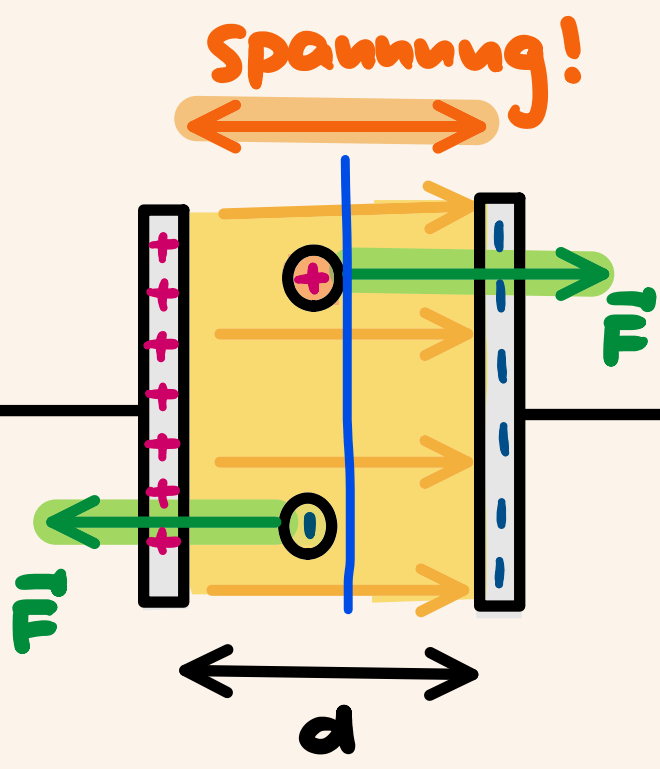
\includegraphics[width = 15 mm]{src/images/hom_potentialfeld.png}
                    \end{center}
                \end{footnotesize}
            \end{minipage}
            \begin{minipage}{0.58\linewidth}
                \begin{scriptsize}
                    \begin{center}
                        \mathbox{
                            U = E\cdot d
                        }
                        Auf \colorbox{Cyan}{Linie} stets selbes Potential/Spannung
                    \end{center}
                \end{scriptsize}
            \end{minipage}
            \vspace{1mm}